%%%%%%%----------------------------------------------------%%%%%%%%%%%%%
\section{Introduction}
\begin{figure}[ht!]
\label{figmot}
\begin{center}
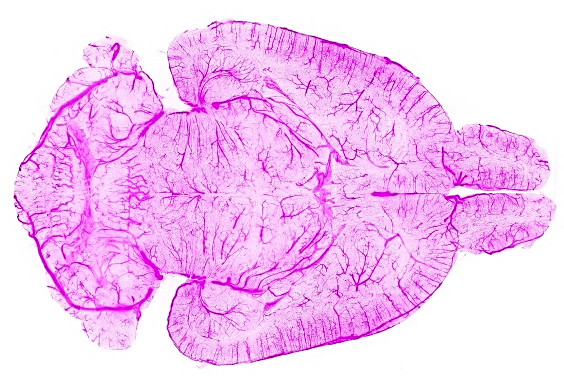
\includegraphics[width=0.44\textwidth]{figs/suppl/3d_vessels.png}
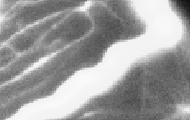
\includegraphics[width=0.15\textwidth]{figs/real.png}
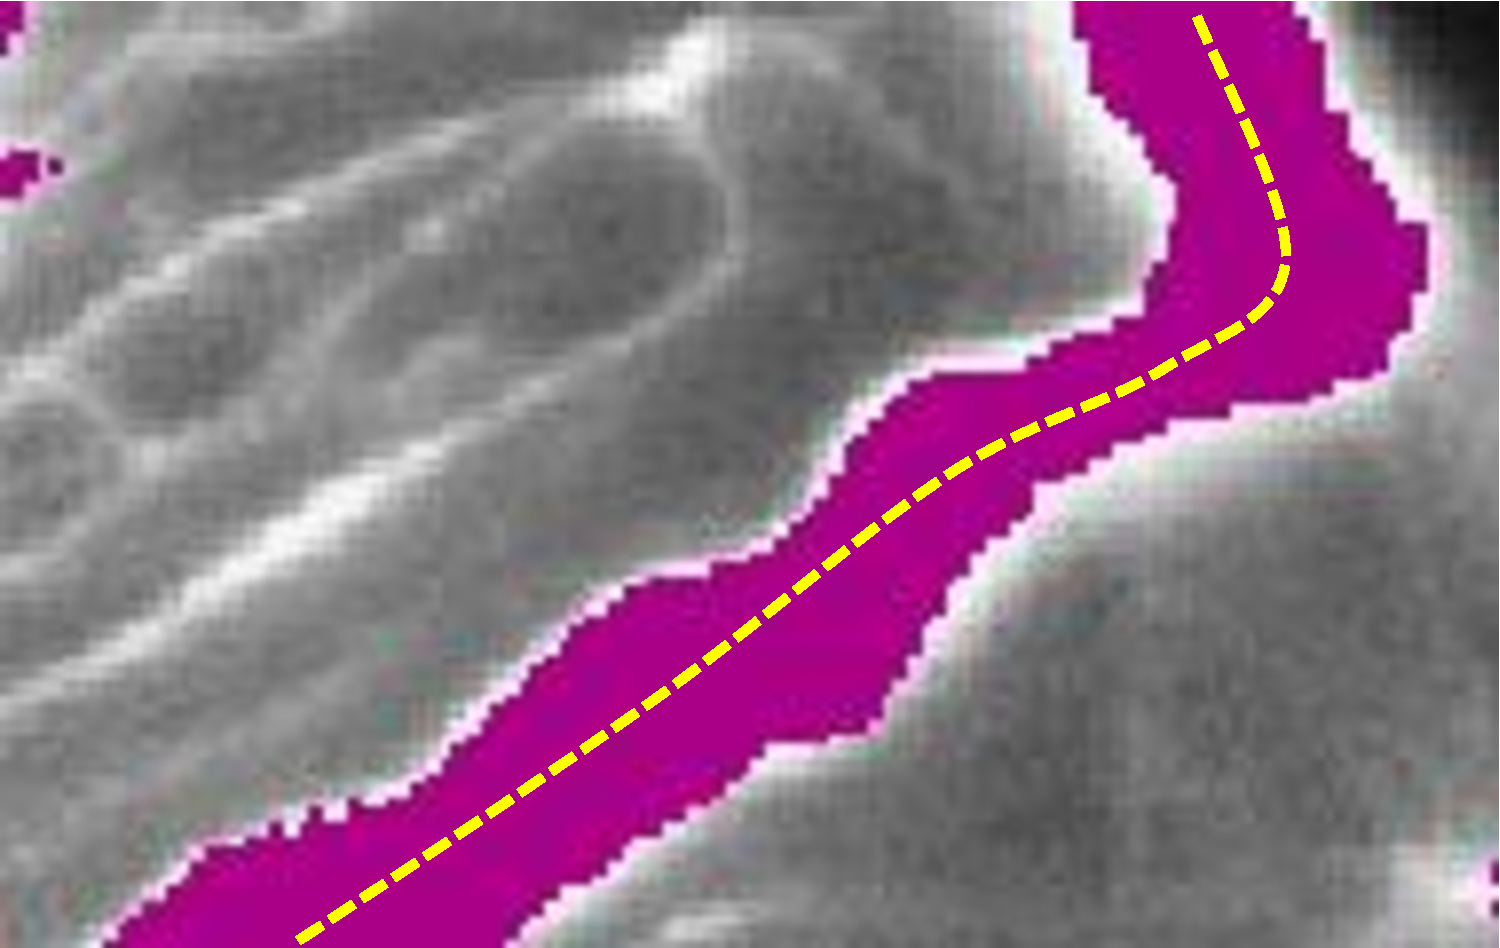
\includegraphics[width=0.15\textwidth]{figs/clDice_fig1_thick.pdf}
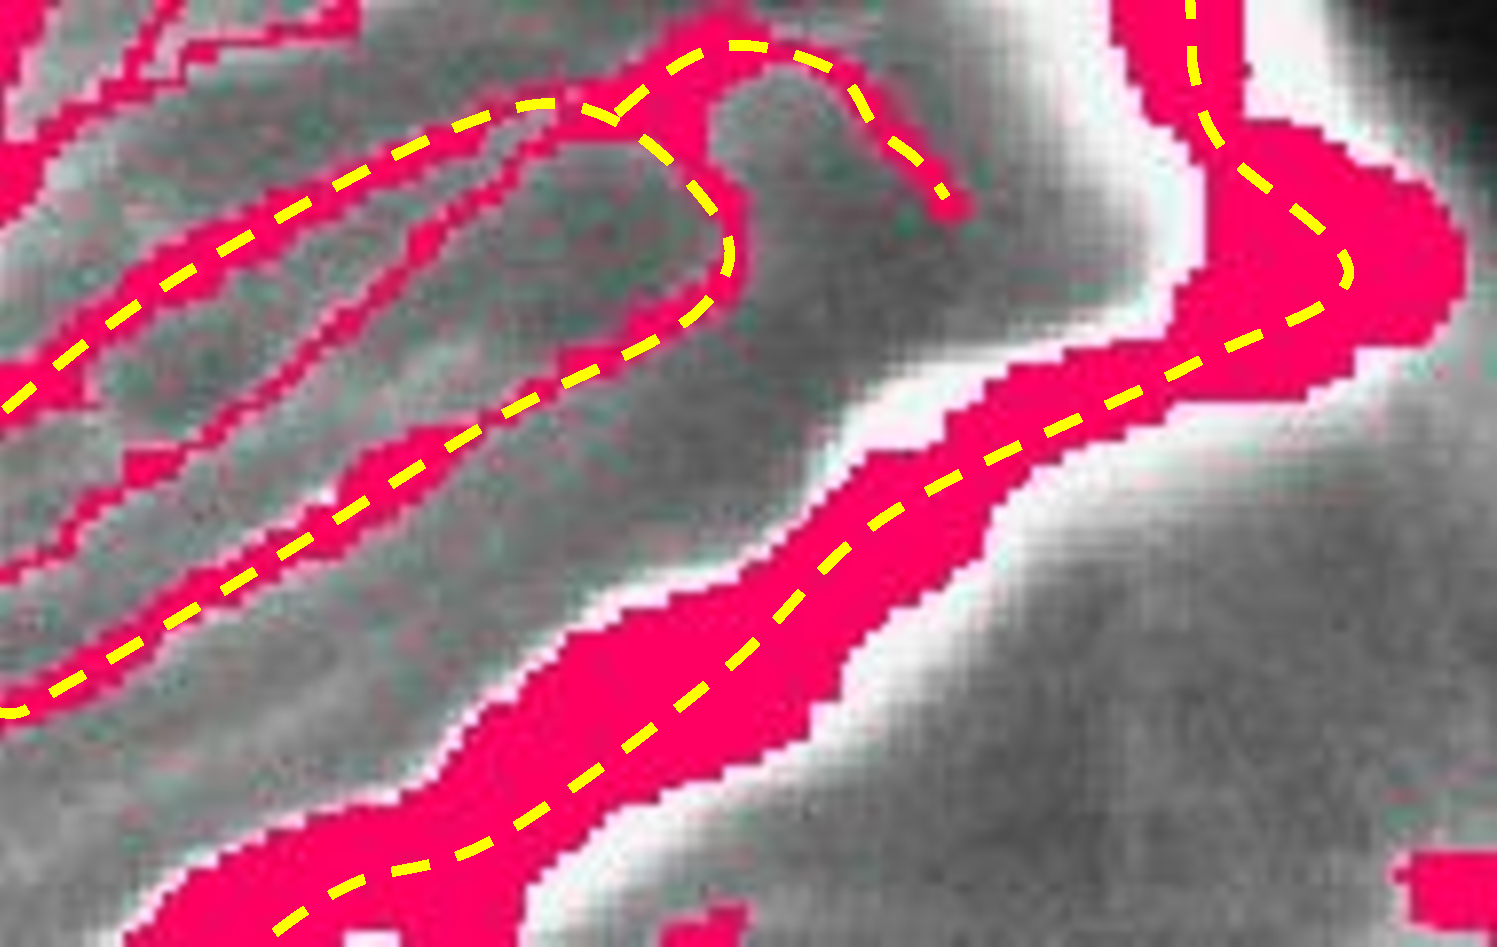
\includegraphics[width=0.15\textwidth]{figs/clDice_fig1_thin.pdf}
\end{center}
\caption{\textbf{Motivation:} The figure shows a 3D rendering of a complex, whole brain vascular dataset \cite{todorov2019automated}, where an exemplary 2D slice of the data is chosen and segmented by two different models, see purple (middle) and red (right), respectively. The two segmentation results achieve identical quality in terms of the traditional Dice score. Note that the purple segmentation does not capture the small vessels while segmenting the large vessel very accurately; on the other side, the red segmentation captures all vessels in the image while being less accurate on the radius of the large vessel. Skeleta are drawn in yellow. From a topology or network perspective, the red segmentation is evidently preferred.}
\vspace{-1.5em}
\end{figure}
Segmentation of \textit{tubular} and \textit{curvilinear} structures is an essential problem in numerous domains, such as clinical and biological applications (blood vessel and neuron segmentation from microscopic, optoacoustic, or radiology images), remote sensing applications (road network segmentation from satellite images) and industrial quality control, etc. In the aforementioned domains, a topologically accurate segmentation is necessary to guarantee error-free down-stream tasks, such as computational hemodynamics, route planning, Alzheimer's disease prediction \cite{hunter2012morphological}, or stroke modeling \cite{joutel2010cerebrovascular}. When optimizing computational algorithms for segmenting curvilinear structures, the two most commonly used categories of quantitative performance measures for evaluating segmentation accuracy of \textit{tubular} structures, are 1) overlap based measures such as Dice, precision, recall, and Jaccard index; and 2) volumetric distance measures such as the Hausdorff and Mahalanobis distance \cite{kirbas2004review,schneider2015joint,phellan2017vascular,hu2018retinal}.

However, in most segmentation problems, where the object of interest is 1) locally a \textit{tubular} structure and 2) globally forms a \textit{network}, the most important characteristic is the connectivity of the global network topology. Note that \textit{network} in this context implies a physically connected structure, such as a vessel network, a road network, etc., which is also the primary structure of interest for the given image data. As an example, one can refer to brain vasculature analysis, where a missed vessel segment in the segmentation mask can pathologically be interpreted as a stroke or may lead to dramatic changes in a global simulation of blood flow. On the other hand, limited over- or under-segmentation of vessel radius can be tolerated, because it does not affect clinical diagnosis.

For evaluating segmentations in such tubular-network structures, traditional volume-based performance indices are sub-optimal. For example, Dice and Jaccard rely on the average voxel-wise hit or miss prediction \cite{taha2015metrics}. In a task like network-topology extraction, a spatially contiguous sequence of correct voxel prediction is more meaningful than a spurious correct prediction. This ambiguity is relevant for objects of interest, which are of the same thickness as the resolution of the signal. For them, it is evident that a single-voxel shift in the prediction can change the topology of the whole network. Further, a globally averaged metric does not equally weight tubular-structures with large, medium, and small radii (cf. Fig~\ref{figmot}). In real vessel datasets, where vessels of wide radius ranges exist, e.g. 30 $\mu$m for arterioles and 5 $\mu$m for capillaries \cite{todorov2019automated,di2018whole}, training on a globally averaged loss induces a strong bias towards the volumetric segmentation of large vessels. Both scenarios are pronounced in imaging modalities, such as fluorescence microscopy \cite{todorov2019automated,zhao2020cellular} and optoacoustics, which focus on mapping small capillary structures. 

To this end, we are interested in a topology-aware image segmentation, eventually enabling a correct network extraction. Therefore, we ask the following research questions: 
%%%%%%%%%%%%%-------------------------------------%%%%%%%%%%%%%%%%%
\begin{enumerate}
    \item[Q1.] What is a good pixelwise measure to benchmark segmentation algorithms for \textbf{tubular}, and related linear and curvilinear structure segmentation while guaranteeing the preservation of the \textbf{network-topology}? 
    \item[Q2.] Can we use this \textit{improved measure} as a loss function for neural networks, which is a void in existing literature?
\end{enumerate}
%%%%%%%%%%%%%-------------------------------------%%%%%%%%%%%%%%%%%
\subsection{Related Literature}
Achieving topology preservation can be crucial to obtain meaningful segmentation, particularly for elongated and connected shapes, e.g. vascular structures or roads. However, analyzing preservation of topology while simplifying geometries is a difficult analytical and computational problem \cite{edelsbrunner2010computational,edelsbrunner2000topological}.

For binary geometries, various algorithms based on thinning and medial surfaces have been proven to be topology-preserving according to varying definitions of topology \cite{kong1995topology,lee1994building,ma1994topology,palagyi20023}. For non-binary geometries, existing methods applied topology and connectivity constraints onto variational and Markov random field-based methods: tree shape priors for vessel segmentation \cite{stuhmer2013tree}, graph representation priors to natural images \cite{andres2011probabilistic}, higher-order cliques which connect superpixels \cite{wegner2013higher} and adversarial learning for road segmentation \cite{vasu2020topoal}, integer programming to general curvilinear structures \cite{turetken2016reconstructing}, and proposed a tree-structured convolutional gated recurrent unit \cite{kong2020learning}, morphological optimization \cite{gur2019unsupervised}, among others \cite{araujo2019deep,han2003topology,nowozin2009global,navarro2019shape,oswald2014generalized,rempfler2017efficient,segonne2008active,vicente2008graph,zeng2008topology,wu2016deep}. Further, topological priors of containment were applied to histology scans \cite{bentaieb2016topology}, a 3D CNN with graph refinement was used to improve airway connectivity \cite{jin20173d}, and recently, Mosinska et al. trained networks which perform segmentation and path classification simultaneously \cite{mosinska2019joint}. Another approach enables the predefinition of Betti numbers and enforces them on the training\cite{clough2020topological}.
%%%%%%%%%%%%%-------------------------------------%%%%%%%%%%%%%%%%%

The aforementioned literature has advanced the communities understanding of topology-preservation, but critically, they do not possess end-to-end loss functions that optimize topology-preservation. %Minimizing a topology-preserving loss function guarantees a perfect topology of a segmentation mask. 
In this context, the literature remains sparse. Recently, %have directly implemented topology-aware loss functions for structure segmentation in CNNs.
Mosinska et al. suggested that pixel-wise loss-functions are unsuitable and used selected filter responses from a VGG19 network as an additional penalty \cite{mosinska2018beyond}. Nonetheless, their approach does not prove topology preservation. Importantly, Hu et al. proposed the first continuous-valued loss function based on the Betti number and persistent homology \cite{hu2019topology}. However, this method is based on matching critical points, which, according to the authors makes the training very expensive and error-prone for real image-sized patches \cite{hu2019topology}. While this is already limiting for a translation to large real world data set, we find that none of these approaches have been extended to three dimensional (3D) data.
%%%%%%%%%%%%%-------------------------------------%%%%%%%%%%%%%%%%%


\subsection{Our Contributions}
The objective of this paper is to identify an efficient, general, and intuitive loss function that enables topology preservation while segmenting tubular objects. 
We introduce a novel connectivity-aware similarity measure named \textit{clDice} for benchmarking tubular-segmentation algorithms. 
Importantly, we provide theoretical guarantees for the topological correctness of the \textit{clDice} for binary 2D and 3D segmentation. As a consequence of its formulation based on morphological skeletons, our measure pronounces the network's topology instead of equally weighting every voxel.
Using a differentiable soft-skeletonization, we show that the \textit{clDice} measure can be used to train neural networks. 
We show experimental results for various 2D and 3D network segmentation tasks to demonstrate the practical applicability of our proposed similarity measure and loss function.